%% %%%%%%%%%%%%%%%%%%%%%%%%%%%%%%%%%%%%%%%%%%%%%%%%
%% Problem Set/Assignment Template to be used by the
%% Food and Resource Economics Department - IFAS
%% University of Florida's graduates.
%% %%%%%%%%%%%%%%%%%%%%%%%%%%%%%%%%%%%%%%%%%%%%%%%%
%% Version 1.0 - November 2019
%% %%%%%%%%%%%%%%%%%%%%%%%%%%%%%%%%%%%%%%%%%%%%%%%%
%% Ariel Soto-Caro
%%  - asotocaro@ufl.edu
%%  - arielsotocaro@gmail.com
%% %%%%%%%%%%%%%%%%%%%%%%%%%%%%%%%%%%%%%%%%%%%%%%%%

\documentclass[12pt]{article}
\usepackage{design_ASC}

\theoremstyle{definition}
\usepackage{longtable}
\newtheorem{exmp}{Example}[section]
\newtheorem{slo}{Definition}[section]
\newcommand*{\Perm}[2]{{}^{#1}\!P_{#2}}%
\newcommand*{\Comb}[2]{{}^{#1}C_{#2}}%
\setlength\parindent{0pt} %% Do not touch this
\usepackage{amsmath}% http://ctan.org/pkg/amsmath
%% -----------------------------
%% TITLE
%% -----------------------------
\title{\textbf{Discrete Random variable}} %% Assignment Title

\author{\textbf{Ibrahim Abou Elenein}}

\date{\today} %% Change "\today" by another date manually
%% -----------------------------
%% -----------------------------

%% %%%%%%%%%%%%%%%%%%%%%%%%%
\begin{document}
\setlength{\droptitle}{-5em}    
%% %%%%%%%%%%%%%%%%%%%%%%%%%
\maketitle
\tableofcontents
\pagebreak
% --------------------------
% Start here
% --------------------------

% %%%%%%%%%%%%%%%%%%%
\section{Random Variable}
A random variable is a quantity “X ” resulting from an experiment, by chance,
that can assume different values.\\

A random variable is a variable “X” that
has a single numerical value determined by chance, for each outcome of a
procedure.\\

If a sample space S is discrete, then every R.V.  defined on S is
also discrete, i.e., its range is countable (think of random counts for
examples).
\section{Discrete Random Variable}
A Discrete Random Variable is a variable that can assume only certain clearly
separated values. \\

A Discrete Random Variable has either a finite or countable
number of values, where “countable” refers to the fact that there might be
infinitely many values, but they can be associated with a counting process.
\subsection{Examples of Discrete Random Variables}
\begin{itemize}
    \item The outcome of rolling a single die.
    \item The number of boys in a family with three children.
    \item The number of heads that appear when a coin is flipped nine times.
    \item The sum of the numbers on the dice, when k dice are rolled.
    \item The number of bits received in error when n bits are received.
    \item The number of bits received until the r-th error.
\end{itemize}
\section{Discrete Probability Distributions}
A discrete probability distribution is a listing of 
all possible values of a random variable along 
with their probabilities. \\
\begin{equation}
    \displaystyle \frac{X}{P(X)} \frac{|x_1|}{|p_1|} \frac{|x_2|}{|p_2|} \frac{|x_2|}{|p_2|} 
    \frac{|\dots|}{|\dots|} \frac{|x_k|}{|p_k|}; \  \ \  \sum _{k \geq 1} p_k = 1.
\end{equation}    
\begin{enumerate}
    \item The sum of all probabilities must be 1in any probability distribution
    \item All probability values must be in [0,1]
\end{enumerate}
\begin{exmp}
    x $\Rightarrow$ The number of heads appearing when a coin is flipped three times.

\end{exmp}

% Please add the following required packages to your document preamble:
% Note: It may be necessary to compile the document several times to get a multi-page table to line up properly
\begin{longtable}[c]{lllll}
    X    & 0   & 1   & 2   & 3   \\
    \endfirsthead
    %
    \endhead
    %
    P(X) & 1/8 & 3/8 & 3/8 & 1/8
\end{longtable}

\subsection{Bernoulli}
A Bernoulli trail is an experiment with only two outcomes Success and Failure 
\begin{enumerate}
    \item $P(S) = p = $ Probability of a success
    \item $P(F) = q = 1 - p = $ Probability of a failure
\end{enumerate}
If a Bernoulli random variable, X, denotes No. of successes, then
\begin{enumerate}
    \item $ X = 1$ if the outcome is success
    \item $ X = 0$ if the outcome is failure
\end{enumerate}
\begin{exmp}
    A bit is transmitted, it is received in error with probability “0.1”.\\
    Assume that 8 bits are transmitted independently.
    \begin{enumerate}
        \item How many bits can be received in error?
            \begin{center}
                $\Perm{8}{2}$
            \end{center}   
        \item What is the probability that 2 bits are received in error
            \begin{center}
                $P(X=2) = \Perm{8}{2} \times (0.1)^2 (0.9)^6  $  
            \end{center}   
    \end{enumerate}
\end{exmp}    
\subsection{Binomial Distribution}
In general, let X stand for the number of bits received in error, when $n$ bits are transmitted,
with the probability of a single bit in error being $p$
\begin{equation}
    P (X = k) = \Comb{n}{k} \times p^k \times (1-p)^{n - k} 
\end{equation}    

\begin{equation}
    \sum_{k = 0}^{n} p_k  = \Comb{n}{k} \times p^k \times (1-p)^{n - k} = [(p)+(1-p)]^n = 1 ^ n = 1
\end{equation}    
\begin{exmp}
    A fair coin is tossed 10 times, what is the probability of getting:
    \begin{enumerate}
        \item  Exactly 6 heads.
            \begin{center}
                $ n = 10; \ \ p = 0.5; q = 0.5 $ 
            \end{center}   
            \begin{center}
                $P(X = 6) = \Comb{10}{6} \times (0.5)^6 \times (0.5)^4   $ 
            \end{center}   
        \item  At least 6 heads.
            \begin{center}
                $P(X \geq 6) = P(X = 6) + P(X = 7) + P(X = 8) + P(X = 9) + P(X = 10)  $
            \end{center}   
    \end{enumerate}
\end{exmp}    

\subsection{Geometric Distribution}

A bit is transmitted, it is received in error with probability “0.1”.

Assume that bits are transmitted independently, until the first bit is received
in error.
\begin{enumerate}

    \item How many bits can be received?
        \begin{center}
            Infinity many many
        \end{center}
    \item What is the probability that the 5-th bit is received in error?
        \begin{center}
            $  P(X = 5) = 0.1 \times 0.9^4 $
        \end{center}
    \item What is the probability that at least 5 (i.e. 5 or more) bits are received until the first error
        \begin{center}
            $  P(X \geq 5) = P(X = 5) + P(X = 6) + \dots $  =
        \end{center}
        \begin{center}
            $  \displaystyle \sum_{k = 5}^{\infty} P(X = K) = \sum_{k = 5}^{\infty}(0.1)(0.9)^{k-1} = 0.656$
        \end{center}

\end{enumerate}
So The General case is 
\begin{equation}
    P(X = k) = p \times (1 - p)^{k-1} ; \ \ \ k \geq 1
\end{equation}    

\begin{equation}
    \displaystyle \sum_{k = 1}^{\infty}   P(X = k) = \sum_{k = 1}^{\infty}p \times (1 - p)^{k-1}
    = p\sum_{k = 1}^{\infty}(1 - p)^{k-1} = p \times \frac{1}{p} = 1
\end{equation}    
\begin{exmp}
    Given that the first $k$ trials were Failures. Find the probability that $(k+1)$-th trial will be a Success. \\

    we need to find that $P(X = k + 1 | X > k)$
    \begin{center}
        $ \displaystyle  P(X = k + 1 | X > k) = \frac{P(X=k+1 \cap X>k)}{P(X>k)}
        = \frac{p \times (1-p)^k}{(1-p)^k} = p = p(X = 1)$  this called lack of memory where the probability
        of k + 1 is the same as the first
    \end{center}
\end{exmp}    
\subsection{Negative Binomial}
When a bit is transmitted, it is received in error with probability “0.1”.
Assume that bits are transmitted independently, until FOUR bits are received in error.
\begin{enumerate}
    \item At least, how many bits can be received ?
        \begin{center}
            at least 4 bits.
        \end{center}   
    \item What is the probability that exactly 10 bits will be received
        \begin{center}
            $  P(X= 10) = (0.1)^9 \times \Comb{9}{3} \times (0.9)^6 \times (0.1)^3 $
        \end{center}   
        In General, $P(X = k) = \Comb{k-1}{3} \times (1-p)^{k-4} \times p^4$

\end{enumerate}   
\begin{slo}
    In general, let X stand for the number of bits
    received until r bits are received in error, with
    the probability of a single bit in error being p.
\end{slo}   
\begin{equation}
    P(X = k) =  \underbrace{p^r}_{\text{last trial}} 
    \ \ \underbrace{\Comb{k-1}{r-1} (1-p)^{k-r}}_{\text{$(r - 1)$success in$(k - 1)$trial}}; \ \ k \geq r. 
\end{equation}
\begin{equation}
    \displaystyle \sum_{k=r}^{\infty} \Comb{k-1}{r-1} p^r(1-p)^{k-r} =
    \sum_{k' = 0}^{\infty} \Comb{k' + r -1}{k'} \ p^r (1-p)^{k'}
\end{equation}
given that $ \displaystyle \Comb{n}{k} = \Comb{n}{n- k}$

\begin{equation}
    \displaystyle \sum_{k' = 0}^{\infty} \Comb{k' + r -1}{k'} \ p^r (1-p)^{k'} =
    p^r \sum_{k'= 0}^{\infty}  \Comb{k' + r-1}{r-1}(1-p)^{k'}
\end{equation}
given that $ \displaystyle \frac{1}{(1-x)^r} = \sum_{k=0}^{\infty} \Comb{k+r-1}{r-1}x^r $
\begin{equation}
    \displaystyle p^r \sum_{k'= 0}^{\infty}  \Comb{k' + r-1}{r-1}(1-p)^{k'} = p^r * \frac{1}{(1-(1-p))^r} = 1 
\end{equation}
\section{Notes}
\begin{enumerate}
    \item Recall that a binomial random variable is a count of the number
        of successes in n Bernoulli trials. That is, the number of trials n is
        predetermined, and the number of successes represents the random variable X.
    \item  A negative binomial random variable is a count of the number of
        trials required to obtain r successes. That is, the number of
        successes r is predetermined, and the number of trials (n or k)
        represents the random variable X.
\end{enumerate}    

\section{Probability Mass Function}
Using the probability distribution “PD” of a discrete RV,
X, with possible values $x_1, x_2\dots, x_n.$ A probability mass function is a function defined such that:
\begin{enumerate}
    \item \[    f(X_k) = P(X = x_k) = p_k,  \]
    \item \[          f(x_k) \geq 0,  \]
    \item \[  \displaystyle \sum_{k=1}^{n} f(x_k) = 1.       \]
\end{enumerate}
Example :\[ f(x)= \begin{cases} 
    p_k, & x=x_k \\
    0, & otherwise
\end{cases}
\] $f$ is a function that is non-trivial only on the range of $X$.

\begin{center}
    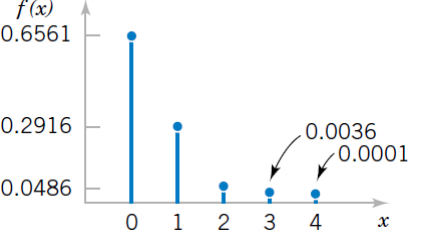
\includegraphics[width=201px]{2.png}
\end{center}
\section{Cumulative Probability Function}
The following function provides an alternative definition for X.
The cumulative probability function of a DRV X is defined by:
\[
    \displaystyle F(x) = P(X \leq x) = \sum_{x_k \leq x}f(x_k)
\]
\[ F(x)= \begin{cases} 
    0, & x < x_1 \\
    p_1, & x_1 \leq x < x_2 \\
    p_1 + p_2, & x_2 \leq x < x_3 \\
    \dots
\end{cases}
\]
\begin{center}
    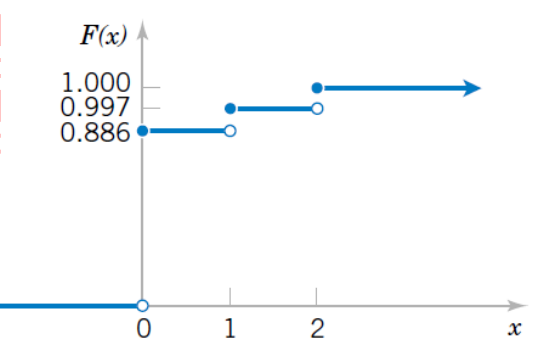
\includegraphics[width=200px]{3.png}
\end{center}
\subsection{Notes}
\begin{enumerate}
    \item $F$ is a step function
    \item $  0 \leq F(X) \leq 1   $
    \item if $x \leq y \Rightarrow F(x) \leq F(y)$
\end{enumerate}
\section{Average of a Discrete Random Variable}
\begin{itemize}
    \item Each time a random experiment is carried out, an associated RV takes on a
        value. Is it possible find an “average” value of the RV ?
    \item For instance, on average, how many bits are received in error
        when 8 bits are transmitted?
    \item Or, on average, how many bits must be received until the first (the
        r-th) error occurs?
        \begin{itemize}
            \item Note that in both cases, you can take a sample, i.e. repeat the
                respective experiment several times and take the value of the
                RV each time.
            \item An average computed this way is, however, dependent on the samle!
            \item Is it possible to get a sample independent value?
        \end{itemize}
\end{itemize}
\section{Expectation}
The expected value, or expectation, of a discrete random variable $X$ is given by
\[
    \displaystyle \mu = E(X) = \sum X *P(X) = \sum_k x_k p_k
\]
The formula gives a weighted average of values
of a random variable, with the probabilities being
the weights of the respective values.
(One can see that the expected value as a weighted probability).
\section{Variance and Standard Deviation}
The average spread of a DRV around its expectation is called the standard
deviation, and is computed via the so-called \textsc{variance}

\[
    \displaystyle \sigma^2 = V(X) = \sum_k  [(x_k -\mu)^2.p_k]\ \ \  \text{or} = 
\]  
\[
    \displaystyle [\sum_k x^2_k.p_k] - \mu^2 = E(X^2) - [E(X)]^2
\]
Standard Deviation is $\sigma = \sqrt{\sigma^2}$
\begin{exmp}
    Compute the mean and the standard deviation of the number of girls in a family with 3 children.\\

    \ \ \ \   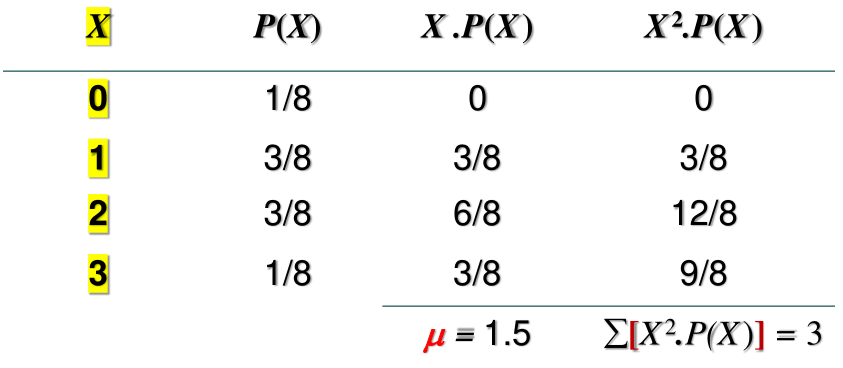
\includegraphics[width=400px]{4.png}
    \[
        \sigma = \sqrt{\sigma^2} = \sqrt{[\sum X^2.P(X)]- \mu^2} = \sqrt{3-(1.5)^2}
    \]
\end{exmp}
\subsection{Expectation and Variance of Bernoulli Random Variable}
\begin{longtable}[c]{l|l|l}
    X    &  1   & 0   \\ \hline 
    \endfirsthead
    %
    \endhead
    %
    P(X) & p&  q
\end{longtable}
\[
    \mu = 1.p + 0(1-p) = p
\]
\[
    \sigma^2 = [1^2.p + 0^2(1-p)] - p^2 = p(1-p) = pq.
\]
\subsection{Expectation and Variance of the Binomial RV}
For a binomial RV with parameters n and p we have:
\[
    \mu = np, 
\]
\[
    \sigma^2 = np(1-p) = npq.
\]
\begin{exmp}
    The Statistical Bulletin published by Metropolitan Life Insurance Co.
    reported that 2\% of all American births result in twins. If a random
    sample of 8000 births is taken, find the mean, variance, and standard
    deviation of the number of births that would result in twins.
    \[
        X \Rightarrow \text{The number of births that would result in twins}
    \]
    \[
        S \Rightarrow \text{twins}; \ \ F \Rightarrow \text{not twins}
    \]
    \[
        n = 8000; p = 0.2; q = 0.98 
    \]
    \[
        \mu = n.p = 8000 \times 0.02 
    \]
    \[
        \sigma^2 = n.p.q = (8000) \times (0.02) \times (0.98) = 156.8 \Rightarrow \sigma = 12.5
    \]
\end{exmp}    
\subsection{Expectation and Variance of the Geometric r.v}
For a geometric RV with parameter p we have:
\[
    \mu = \frac{1}{p}.
\]
\[
    \sigma^2 = \frac{1-p}{p^2} = \frac{q}{p^2}.
\]
\end{document}
